\documentclass[tikz]{standalone}
\usepackage{tikz}
\usetikzlibrary{positioning, graphs}
\usetikzlibrary{graphs.standard}
\begin{document}
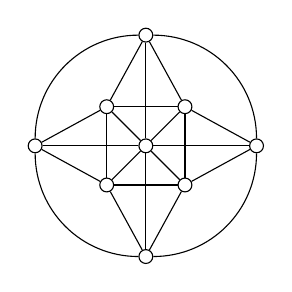
\begin{tikzpicture}
		[every node/.style={draw,circle,inner sep = 0mm, minimum size = 0.5em}]
		\graph[clockwise, radius = 4em, phase = 0, empty nodes]{subgraph I_n[n = 4, name = A]};
		\graph[clockwise, radius = 2em, phase = -135, empty nodes] {subgraph C_n [n = 4, name = B]};
		
		\draw (0,0) node (a) {};
		
		\draw (A 1) to [in = 0, out = -90] (A 2);
		\draw (A 2) to [in = -90, out = 180] (A 3);
		\draw (A 3) to [in = 180, out = 90] (A 4);
		\draw (A 4) to [in = 90, out = 0] (A 1);
		
		\foreach \i [evaluate={\j=int(mod(\i+1,4)+1); \k=int(mod(\i+2,4)+1);}] in {1, 2, 3, 4}{
			\draw (A \i) -- (a);
			\draw (B \i) -- (a);
			\draw (A \i) -- (B \k);
			\draw (B \i) -- (A \j);
		}
\end{tikzpicture}
\end{document}